\documentclass{llncs}
\usepackage{hyperref}
\usepackage{tikz}
\usetikzlibrary{shapes,arrows,patterns}
\usepackage{subcaption}
\usepackage{pifont}
\usepackage{graphicx}

\newcommand{\vampire}{{Vampire}}
\newcommand{\iprover}{iProver}
\newcommand{\E}{{\textsc E}}
\newcommand{\zthree}{{\textsc Z3}}
\newcommand{\tick}{\ding{51}}
\newcommand{\cross}{\ding{55}}
\newcommand{\todo}[1]{{\color{red} #1}}

\title{Dynamic Strategy Priority: \\ Empower the strong and abandon the weak.}
\titlerunning{Dynamic Strategy Priority}
\authorrunning{Rawson and Reger}
\author{
 Michael Rawson \and 
 Giles Reger
}
\institute{
University of Manchester, Manchester, UK
}

\begin{document}
\maketitle
\begin{abstract}
Automated theorem provers are often used in other tools as black-boxes for discharging proof obligations. One example where this has enjoyed a lot of success is within interactive theorem proving. 
%
A key usability factor in such settings is the time taken for the provers to complete.
Automated theorem provers typically run lists of proof strategies sequentially, which can cause proofs to be found more slowly than necessary if the ordering is suboptimal.
We show that it is possible to predict which strategies are likely to succeed while they are running using an artificial neural network.
We also implement a run-time strategy scheduler in the \vampire{} prover which utilises a trained neural network to improve average proof search time, and hence increases usability as a black-box prover.
\end{abstract}

%%%%%%%%%%%%%%%%%%%%%%%%%%%%%%%%%%%%%%%%%%%%%%%%%%%%%%%
\section{Introduction}
\label{sec:intro}
%
Modern automated theorem provers (e.g. \E{}~\cite{E}, \iprover{}~\cite{iProver}, \vampire{}~\cite{Vampire}, CVC4~\cite{CVC4}) for first-order logic rely on \emph{portfolio modes}~\cite{portfolio}, which utilise tens to hundreds of distinct \emph{strategies}.
Of these strategies, only a few might solve a hard problem, often rapidly.
Typically, a portfolio of strategies has a pre-defined execution order: the prover will process strategies in this order, running each until a winning strategy is found or the prover runs out of time or strategies.

Portfolio modes are important as, in practice, there is no best strategy.
Furthermore, it is uncommon that two hard problems are efficiently solved by the same strategy.
However, portfolio execution is not without problems: deciding the optimal ordering and time allocation is hard in general~\cite{predict-success}, and produces overly-rigid, brittle engineering when applied to specific domains, such as those found in the TPTP problem set~\cite{TPTP}.
Moreover, for any particular problem, some lengthy strategies that are successful on other problems are doomed to failure from the outset --- as illustrated in Figure \ref{fig:blocking} --- but are left to run unchecked by the prover, wasting time that could be spent on more productive strategies.

\begin{figure}
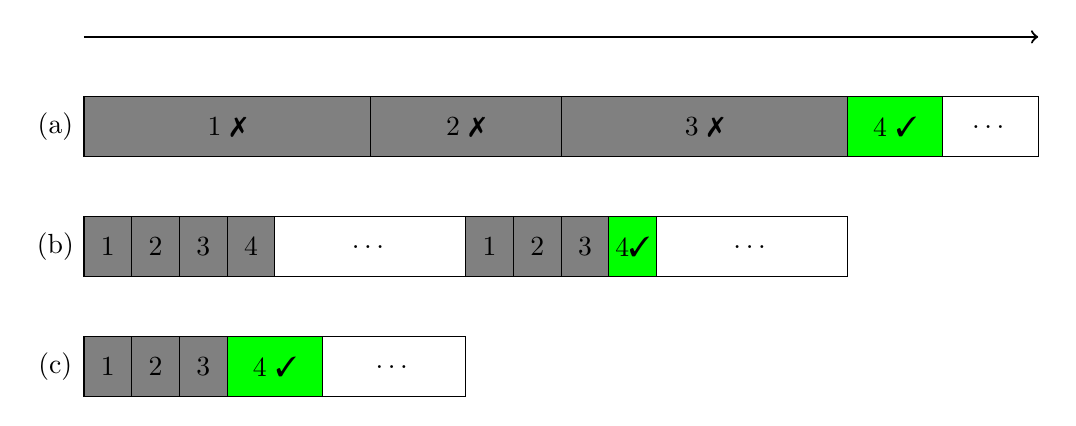
\begin{tikzpicture}[x=0.01\textwidth, y=.3in]
	\draw[thick, ->] (0, 6) -- (100, 6) node {};

	\draw (-3, 4.5) node {(a)};
	\draw[fill=gray] (0, 4) rectangle (30, 5) node [midway] {1 \cross};
	\draw[fill=gray] (30, 4) rectangle (50, 5) node [midway] {2 \cross};
	\draw[fill=gray] (50, 4) rectangle (80, 5) node [midway] {3 \cross};
	\draw[fill=green] (80, 4) rectangle (90, 5) node [midway] {4 \tick};
	\draw (90, 4) rectangle (100, 5) node [midway] {\ldots};

	\draw (-3, 2.5) node {(b)};
	\draw[fill=gray] (0, 2) rectangle (5, 3) node [midway] {1};
	\draw[fill=gray] (5, 2) rectangle (10, 3) node [midway] {2};
	\draw[fill=gray] (10, 2) rectangle (15, 3) node [midway] {3};
	\draw[fill=gray] (15, 2) rectangle (20, 3) node [midway] {4};
	\draw (20, 2) rectangle (40, 3) node [midway] {\ldots};
	\draw[fill=gray] (40, 2) rectangle (45, 3) node [midway] {1};
	\draw[fill=gray] (45, 2) rectangle (50, 3) node [midway] {2};
	\draw[fill=gray] (50, 2) rectangle (55, 3) node [midway] {3};
	\draw[fill=green] (55, 2) rectangle (60, 3) node [midway] {4\tick};
	\draw (60, 2) rectangle (80, 3) node [midway] {\ldots};

	\draw (-3, 0.5) node {(c)};
	\draw[fill=gray] (0, 0) rectangle (5, 1) node [midway] {1};
	\draw[fill=gray] (5, 0) rectangle (10, 1) node [midway] {2};
	\draw[fill=gray] (10, 0) rectangle (15, 1) node [midway] {3};
	\draw[fill=green] (15, 0) rectangle (25, 1) node [midway] {4 \tick};
	\draw (25, 0) rectangle (40, 1) node [midway] {\ldots};
\end{tikzpicture}
\caption{Several strategy schedules and their effects. (a) Failing strategies might block a successful strategy. (b) Round-robin scheduling can help mitigate this problem. (c) This approach is improved if promising strategies run for longer.}
\label{fig:blocking}
\end{figure}

This work makes two contributions. 
We first demonstrate correlation between trends in dynamic properties of proof search, and the pending success or failure of a strategy (Sections~\ref{sec:data},~\ref{sec:predict}).
We then utilise this to implement strategy scheduling, prioritising those strategies most likely to succeed (Section~\ref{sec:intelligent}).
This approach differs from previous work~\cite{E,static1,static2} which attempts to predict successful strategies \emph{a priori} from static features of the input problem; instead we tip running strategies for success based on dynamic, run-time features and use this information to make decisions at runtime. Our experiments (Section~\ref{sec:experiments}) show that guiding scheduling in this way can significantly speed up portfolio-based approaches. Before introducing these contributions and results we first present necessary background in Sections~\ref{sec:vampire} and~\ref{sec:ml}.

%%%%%%%%%%%%%%%%%%%%%%%%%%%%%%%%%%%%%%%%%%%%%%%%%%%%%%%
\section{Strategies in Vampire}
\label{sec:vampire}
%
Vampire is a first-order superposition theorem prover. 
This section reviews its basic structure and components relevant to the rest of this paper. 
We will use the word \textit{strategy} to refer to a set of configuration parameter values that control proof search and \textit{proof attempt} to refer to a run of the prover using such a strategy.

%%%%%%%%%%%%%%%%%%
\subsection{Input and preprocessing}
%%%%%%%%%%%%%%%%%%

Vampire accepts problems in first-order logic with equality and a pre-defined set of first-order theories (e.g. arithmetic, arrays, datatypes). Vampire typically works with problems in the TPTP format \cite{TPTP} but also accepts problems in SMT-LIB~\cite{smt-lib}. 

Problems are parsed and transformed into a set of input clauses used by the saturation algorithm.
This process involves clausification and a number of preprocessing steps.
These preprocessing steps can alter certain properties of the problem e.g. its size and distribution across the signature, sometimes significantly: for example, the E.T. system~\cite{ET} implements a pre-processor for E which selects small sets of axioms from a larger set, for large-theory reasoning.
This means that any prediction method that relies solely on the input problem (rather than dynamic characteristics such as post-preprocessing properties) will find it harder to predict the best parameters for proof search.

%Some preprocessing steps, such as naming and inequality splitting, can alter the signature. %This is important when it comes to cooperation between proof attempts. 
%Later we will see that cooperation is based on the idea that cooperating proof attempts are exploring different areas of the same search space, this would no longer be true if the original clauses differed. 
%Therefore, this work will assume that sets of strategies are \emph{preprocessing-compatible} i.e. after preprocessing the same set of input clauses are used by each strategy.

%%%%%%%%%%%%%%%%%%
\subsection{Saturation algorithms}
%%%%%%%%%%%%%%%%%%

Superposition provers such as Vampire use \emph{saturation algorithms with redundancy elimination}.
They work with a search space consisting of a set of clauses and use a collection of generating,
simplifying and deleting inferences to explore this space. 
Generating inferences, such as superposition, extend this search space by adding new clauses obtained by applying inferences to existing clauses.
Simplifying inferences, such as demodulation, replace a clause by a simpler one.
Deleting inferences, such as subsumption, delete a clause, typically when it becomes redundant (see \cite{resolutionHandbook}). Simplifying and deleting inferences must satisfy this condition to preserve completeness.

The goal is to \emph{saturate} the clause set with respect to the inference system. If the empty clause is derived then the input clauses are unsatisfiable. If no empty clause is derived and the search space is saturated then the input clauses are guaranteed to be satisfiable \emph{only if} a complete strategy is used. A strategy is complete if it is guaranteed that all inferences between non-deleted clauses in the search space will be applied. Vampire includes many incomplete strategies as they can be very efficient at finding unsatisfiability.

%Completeness relies on a fair \emph{clause selection} strategy
%In Vampire the application of inferences make heavy use of \emph{term indexing}

All saturation algorithms implemented in Vampire belong to the family of \emph{given clause algorithms}, which achieve completeness via a fair \emph{clause selection} process that prevents the indefinite skipping of old clauses. These algorithms typically divide clauses into three sets, \emph{unprocessed}, \emph{passive} and \emph{active}, and follow a simple \emph{saturation loop}:
\begin{enumerate}
	\item Add non-redundant \emph{unprocessed} clauses to \emph{passive}. Redundancy is checked by attempting to \emph{forward simplify} the new clause using processed clauses.
	\item Remove processed (passive and active) clauses made redundant by newly processed clauses, i.e.\ \emph{backward simplify} existing clauses using these clauses.
	\item Select a given clause from \emph{passive}, move it to \emph{active} 
	and perform all generating inferences between the given clause and all other active clauses,
	adding generated clauses to \emph{unprocessed}.
\end{enumerate}
Later we will show how iterations of this saturation loop from different proof attempts can be interleaved. Vampire implements three saturation  algorithms:
\begin{enumerate}
	\item \emph{Otter} uses both passive and active clauses for simplifications.
	\item \emph{Limited Resource Strategy (LRS)} \cite{LRS} extends Otter with a heuristic
	   that discards clauses that are unlikely to be used with the current resources, i.e.\ time and memory.
		 This strategy is incomplete but also generally the most effective at proving unsatisfiability.
	\item \emph{\sc Discount} uses only active clauses for simplifications.
\end{enumerate}
A recent development in Vampire is AVATAR \cite{avatar,playing} which integrates with the saturation loop to perform clause splitting. The general idea is to use a SAT solver to select a subproblem by naming each clause sub-component by a propositional variable, running a SAT solver on these abstracted clauses, and using the subsequent propositional model to select components to include in proof search. 
At the end of each iteration of the loop we check whether the underlying subproblem has changed. AVATAR can occasionally make loops run a little longer, but no more than other steps such as backward subsumption. Otherwise, the notion of saturation loop remains the same when using AVATAR.

There are also other proof strategies that fit into the above loop format 
and can be interleaved with superposition based proof attempts.
For example, instance generation \cite{instgen} saturates the set of clauses with respect to the instance generation rule and finite model finding \cite{Reger2016sat} iteratively checks larger model sizes (these loops tend to be much longer than those from other algorithms).



%%%%%%%%%%%%%%%%%%
\subsection{Strategies in Vampire}
%%%%%%%%%%%%%%%%%%

%A strategy is a set of configuration parameter values that controls proof search.
Vampire includes more than 50 parameters. By only varying parameters and values used by Vampire at the last CASC competition, we obtain over 500 million strategies. These parameters control
\begin{itemize}
	\item Preprocessing steps (24 different parameters)
	\item The saturation algorithm and related behaviour e.g. clause selection
	\item Inferences used (16 different kinds with variations)
	%\item Parameters to control splitting via AVATAR e.g. when it occurs
\end{itemize}
Even restricting these parameters to a single saturation algorithm and straightforward preprocessing steps, the number of possible strategies is vast. For this reason, Vampire implements a portfolio \emph{CASC mode} \cite{Vampire} that categorises problems based on syntactic features and attempts a sequence of approximately 50 strategies over a five minute period (this number can vary significantly). These strategies are the result of extensive benchmarking and have been shown, experimentally, to work well on unseen problems i.e. those not used for training.

The syntactic features used by the current portfolio mode are coarse-grained and include the rough size of the problem (e.g. bucketed into tiny, small, medium, large, huge), the presence of features such as equality or certain theories, and whether the problem is effectively propositional or horn. Not all combinations of these are considered. Portfolio mode is created by considering a set of training data over a list of strategies and attempting to cover as much of it as possible by splitting the set of problems into smaller groups based on these features until all solutions fit into a given time limit. This process is greedy and places the strategy that solves the most problems during training first and then the next best strategy after removing the problems solved by the first solver and so on.

%%%%%%%%%%%%%%%%%%%%%%%%%%%%%%%%%%%%%%%%%%%%%%%%%%%%%%%
\section{Machine Learning and Theorem Proving} \label{sec:ml}

In this section we review the necessary background in machine learning in the context of theorem proving, in particular neural networks.
Other technologies exist which are capable of similar performance, but neural networks produced the best combination of convenience and performance for our purposes.

\subsection{Classification with neural networks}
\emph{Binary classification problems} can be heuristically solved by means of \emph{supervised learning} methods.
A binary classification problem is, informally, the statement ``given input \(X\), does \(X\) belong to class \(A\) or class \(B\)'', where \(X\) is a member of the target domain \(\mathcal{D}\), and \(A, B\) are disjoint subsets of \(\mathcal{D}\) such that \(\mathcal{D} = A \cup B\).
Supervised learning methods attempt to solve binary classification problems by starting with a neutral, untrained heuristic for classifying \(X\) into \(A\) or \(B\), then changing their internal state to improve the heuristic by looking at examples of \(A\) and \(B\) (``training'').
Typically, supervised learning methods do not work on \(X\) directly, but from a set of ``features'' \emph{derived} from \(X\).
Engineering features, or choosing which of a set of supplied features to use, is a field of study in itself.

\begin{figure}[t]
	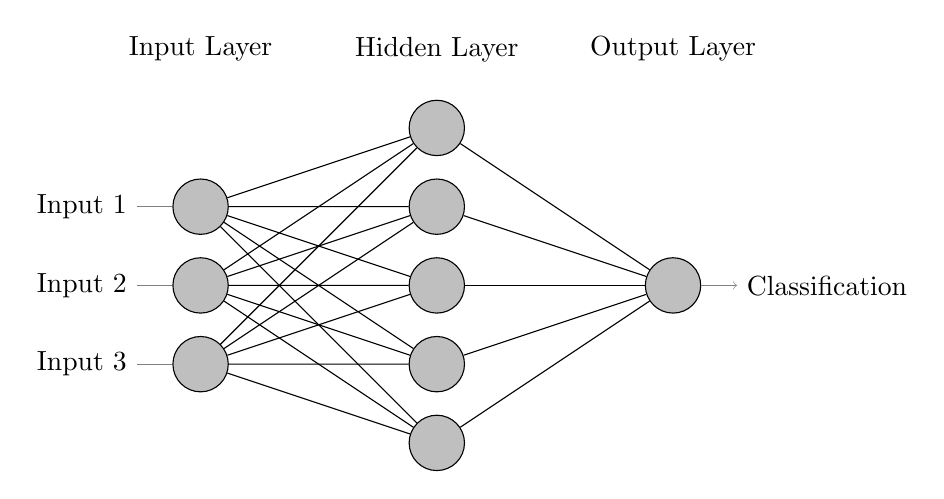
\begin{tikzpicture}[node distance=\layersep]
		\def\layersep{3cm}
		\tikzstyle{neuron} = [circle, draw, fill=black!25, minimum size=20pt]
		% input layer
		\foreach \name / \y in {1, ..., 3}
			\node[neuron, pin=left:Input \name] (input-\name) at (0, -\y cm) {};

		% hidden layer
		\foreach \name / \y in {1, ..., 5}
			\node[neuron, yshift=1cm] (hidden-\name) at (\layersep, -\y cm) {};

		% final layer
			\node[neuron, right of=hidden-3, pin={[pin edge={->}]right:Classification}] (final){};

		% input-hidden connections
		\foreach \source in {1, ..., 3}
			\foreach \target in {1, ..., 5}
				\path (input-\source) edge (hidden-\target);

		% hidden-final connections
		\foreach \source in {1, ..., 5}
			\path (hidden-\source) edge (final);

		% annotations
		\node[text centered, above of=input-1, node distance=2cm] {Input Layer};
		\node[text centered, above of=hidden-1, node distance=1cm] {Hidden Layer};
		\node[text centered, above of=final, node distance=3cm] {Output Layer};
	\end{tikzpicture}
	\centering
	\caption{A neural network with 3 inputs, a single densely-connected hidden layer, and a single output neuron. This is a type of network that might be used for simple binary classification tasks. A version of this architecture with more input and hidden neurons is used for this work.}
	\label{fig:neural-architecture}
\end{figure}
\begin{figure}
	\begin{tikzpicture}[xscale=0.75, yscale=4]
		\draw[->] (-6, 0) -- (6, 0) node[right] {$x$};
		\draw[->] (0, 0) -- (0, 1) node[above] {$\sigma(x)$};
		\draw[blue] (0, 0) plot[domain=-6:6] (\x, {1 / (1 + exp(- \x))});
	\end{tikzpicture}
	\centering
	\caption{The sigmoid function \(\sigma(x) = \frac{1}{1 + e^{-x}}\). This function ``squeezes'' the output to the range \([0, 1]\).}
	\label{fig:sigmoid}
\end{figure}

A neural network consists of a collection of artificial ``neurons'', wired together with connections into a \emph{neural network architecture} (see Figure \ref{fig:neural-architecture} for an example).
Each neuron \(n\) computes a real-valued function \(f_n\), which may be tuned with real-valued parameters: every neuron has a \emph{bias} \(b_n\), and \emph{weight vector} \(\textbf{w}_{n}\).

\(f_n\) is defined on an input vector \(\textbf{x}\) as
\[
	f_n(\textbf{x}) = A\left(\textbf{w}_n\cdot\textbf{x} + b_n\right)
\]

i.e. a weighted sum of all connected input neurons' activation functions, plus the bias of the neuron, all fed through an \emph{activation function} \(A(x)\).
The choice of activation function is dependent on both the position of the neuron in the architecture, and on the target domain: a common choice is the sigmoid function \(\sigma(x)\), as shown in Figure \ref{fig:sigmoid}.

Neural network parameters may be \emph{trained} by a variety of different techniques (randomly, neuro-evolution methods, backpropagation methods, \emph{etc.}).
We used a backpropagation method, which, given a training input \(X\) and correct output \(y\), tunes the network parameters by propagating an error signal backwards through the network to obtain updated parameters for each neuron, hence reducing the error signal for that example~\cite{backpropagation}.
Repeating this process for multiple training examples can produce very good results, but frequently only with the correct combination of learning algorithm, starting weights, network architecture, and training examples.

\subsection{Related work}
Machine learning has potential for significant effect in this area: despite the computational difficulties experienced by theorem provers, frequently proofs have human (or otherwise regular) structure, which may be exploited by the use of learning methods.
The authors are aware of work in the fields of premise selection~\cite{deepmath, mash, malarea, deep-graph-embedding}, static strategy selection~\cite{bridge, males, e-males}, and more recently, direct proof guidance~\cite{malecop, femalecop, deep-proof-search}.
However, we are not aware of any previous work in the area of strategy selection at runtime for conventional theorem provers. The closest area of work is that of static strategy selection where work, with the exception of Bridge et al. \cite{bridge} focusses on static properties of the input problem rather than dynamic properties of the proof search space. Bridge considered various dynamic features of the search space after 100 steps of the saturation algorithm in the default mode (of the E theorem prover \cite{E}).

So far, machine learning techniques have typically used classical machine-learning techniques such as na\"ive Bayesian methods, SVMs~\cite{svm}, and decision trees~\cite{decision-tree}.
However, some newer work has begun to utilise recently-developed deep-neural-network methods~\cite{deepmath, deep-graph-embedding, deep-proof-search}.

%%%%%%%%%%%%%%%%%%%%%%%%%%%%%%%%%%%%%%%%%%%%%%%%%%%%%%%
\section{Feature collection} \label{sec:data}
%
This section discusses which features are extracted from \vampire{} for prediction and how they are extracted. This information is firstly required to identify a correlation and will then be used to train a predictor.

Modifying Vampire to log execution data (such as memory usage, or more specific metrics such as the number of generated clauses) for different strategies obtained from its primary portfolio mode\footnote{CASC-mode, a portfolio designed for the CASC competition~\cite{CASC}.} is straightforward, but some data-collection decisions were made:
\begin{itemize}
	\item Only numerical data immediately available in the prover was collected, but there is scope here for both non-numeric and derivative data sources, which may provide greater insight into the proof state in future work. Suppose that quantities \(A\) and \(B\) are measured directly, but are more often discussed in terms of categories \(C\) that all \(A, B\) pairs fall into. Data could then include \(C\) as well, or instead of, \(A\) and \(B\), embedding \(C\) into the neural network via a one-hot encoding.
	\item Data was collected at intervals of a fixed number of internal resolution steps (in the experiments presented in this paper, this value was 10). This may not necessarily correspond to fixed time intervals, as each step may be more or less expensive, depending on the strategy and the problem.
	\item All available data was collected, even if it emerged to be constant or unhelpful. This allowed an agnostic approach to learning in which the neural network training procedure selected relevant features.
\end{itemize}
In all, 376 features are recorded, including the number of active clauses, passive clauses, and subsumptions, for instance.
The execution traces produced are difficult to work with, however: some are short or non-existent, others are extremely lengthy. The mean execution trace length was 536 (standard deviation: 1208) with the longest trace being 9971 recorded steps long.
Some feature values also have an extremely high variance.
To deal with these problems, a post-processing step is applied.
For each feature, the mean over the entire data set is then mapped to 0, and the dataset is scaled to unit variance.
Data that are too short (fewer than 10 steps) are discarded (the strategy likely did not take very long in any case).
The remaining data is then sliced into 10 evenly-sized ``buckets'', then an average of each bucket is taken to produce 10 values for every trace, and hence a fixed data size.

However, even now these data are not representative of the classification problem desired: these traces show \emph{completed} runs of Vampire, whereas the classifier will be used to predict the success or otherwise of runs of Vampire that are still in progress.
Hence, we take ``snapshots'' at various stages (in these experiments, at every quarter) of the trace, discarding the rest of the data, then post-process the remaining trace as described above.
Conveniently, this also provides 4 times the original number of training examples.
An example post-processed trace is shown in Figure \ref{fig:trace}.

\begin{figure}
	\includegraphics[width=\textwidth]{plot}
	\caption{An example trace, displayed as a colourmap, after post-processing.}
	\label{fig:trace}
\end{figure}

%%%%%%%%%%%%%%%%%%%%%%%%%%%%%%%%%%%%%%%%%%%%%%%%%%%%%%%
\section{Predicting successful strategies} \label{sec:predict}
%
Being able to predict which proof search attempts will succeed in time, and which will fail, based solely on information in the execution trace may seem unlikely.
However, it is known that the ``slowly-growing search space'' maxim, which states that strategies which minimise the number of derived clauses over time are more likely to succeed, is an effective heuristic for finding good strategies in saturation-based theorem proving~\cite{predict-success}.
Since the data we use includes the number of derived clauses, among many other features, it appears more plausible that this approach might work at least as well as the slow-growth heuristic alone.
Engineering a prediction algorithm that attempts to partition traces into ``succeeding'' and ``failing'' classes is possible with the use of modern machine-learning techniques.
Conveniently, these methods do not usually produce a binary output, but instead some \(f(\mathbf{X}) \in \left[0, 1\right]\) which might be seen as the ``level of confidence'' in success of the trace, \(\mathbf{X}\).
This success score can be used to apply an ordering to executing strategies, allowing ``smart'' dynamic scheduling of strategies.

In particular, we evaluated (using the \emph{Keras}~\cite{keras} backend-agnostic neural network suite and the \emph{scikit-learn}~\cite{scikit-learn} utilities)
\begin{enumerate}
	\item A simple neural network with one input for each datum in the trace and a single hidden layer.
	\item A convolutional network~\cite{cnn} which performs a 1-dimensional convolutional pass along the time axis for each feature before the hidden layer.
	\item A recurrent network~\cite{gru}, feeding the time series into a gated recurrent unit before processing.
\end{enumerate}
Results for this classification task are shown in Figure \ref{fig:xvalidation}. The consistent level of accuracy achieved is encouraging. 
Both of the more-advanced classifiers performed better than the simple neural network.
However, the simple network was chosen for integration into Vampire for implementation simplicity, and for performance reasons --- it is ``good enough''. 

\begin{figure}
	\centering
	\begin{tabular}{c c c}
		Method & Mean Accuracy & Standard Deviation\\
		\hline
		Simple neural network & 81.5\% & 2.0\%\\
		Convolutional network & 82.4\% & 3.1\%\\
		Recurrent network & 83.9\% & 1.9\%\\
	\end{tabular}
	\caption{\(k\)-fold cross-validation classification accuracy on a balanced dataset of around 10,000 (total) succeeding and failing execution traces. \(k=5\).}
	\label{fig:xvalidation}
\end{figure}

%%%%%%%%%%%%%%%%%%%%%%%%%%%%%%%%%%%%%%%%%%%%%%%%%%%%%%%
\section{Intelligent scheduling for Vampire} \label{sec:intelligent}
%
We show that this abstract predictor can be used in a concrete implementation for the Vampire prover.
In the modified prover, it is used to run several strategies from Vampire's portfolio in a modified scheduler: strategies self-report their own execution data to the supervisor process and halt for re-evaluation at regular intervals.
When a strategy halts, the scheduler then decides whether to re-schedule the strategy for some more time, or to swap it out for a different strategy.
The algorithm used is as follows, taking as input a set of strategies to run: \
\begin{enumerate}
	\item Initialize an empty ``run pool'' of processes, with a maximum size equal to the desired number of workers (e.g. CPU cores available). Also initialize an empty priority queue of paused processes.
	\item Whenever the pool is under capacity, take the following steps:
	\begin{enumerate}
		\item If the best process in the paused queue has a priority greater than the static priority \(p_\textrm{static}\), wake it and move it into the running pool. In tests, a static priority of around 0.5 appeared to work best.
		\item Otherwise, take a new strategy from the input set and start a new process to run that strategy.
		\item If the input set is empty, take the process from the queue regardless of its priority.
	\end{enumerate}
	\item When a strategy pauses:
	\begin{enumerate}
		\item Remove the process from the pool.
		\item Re-evaluate the process priority using the neural network and the data it provided.
		\item Insert the process into the queue with the computed priority.
	\end{enumerate}
	\item When a strategy terminates, check if it succeeded. Otherwise, remove it from the pool.
	\item If the pool, the queue, and the set of input strategies are all depleted, all strategies have failed. Exit.
\end{enumerate}

To embed the neural network into Vampire, we took the trained network weights from our Python-based experiments, and generated a C source file with these weights included as a large array.
The neural network's architecture was then re-implemented manually in C++, using the network weights compiled into the new program.
This approach had several advantages: while perhaps not as efficient as an architecture such as TensorFlow~\cite{tensorflow} (which may use graphics hardware to accelerate computations), our approach is \emph{reasonably} efficient, but is also low-latency, does not incur any additional dependencies, and does not add significantly to program start-up time.

%%%%%%%%%%%%%%%%%%%%%%%%%%%%%%%%%%%%%%%%%%%%%%%%%%%%%%%
\section{Experimental results} \label{sec:experiments}

We evaluate whether our prediction results carry through to improved performance in Vampire.

\paragraph{Experimental setup} We take all relevant problems for Vampire from TPTP 6.4.0 (17,281 problems in total) and run three variations of Vampire 4.2.1's CASC portfolio mode:
\begin{itemize}
	\item \emph{baseline} was the standard portfolio mode
	\item \emph{no-prediction} uses the dynamic scheduling architecture without prediction. This effectively produces a round-robin scheduling of strategies.
	\item \emph{prediction} uses the trained neural network to predict whether a strategy will be successful as previously described.
\end{itemize}	
The default 3GB memory limit and 300s time limit from the standard portfolio mode were kept but in addition each variation was run in a \emph{multicore} setup using 4 cores to distribute strategies over.Experiments were run on the StarExec cluster \cite{starexec} where each node contains an Intel Xeon 2.4GHz processor. 

\begin{table}[t]
\caption{Results for the three variations.\label{tab:numbers}}
\centering
\begin{tabular}{l|ccccc}
				& Solved & New & Unique & Average time (wall) & Average time (cpu) \\ \hline
\emph{baseline}		& 12,899 &- & 420 & 3.03s $\pm$ 9.91s &10.53s $\pm$ 33.60s\\
\emph{no-prediction}	& 11,827 & 56& 33 & 2.86s $\pm$ 8.33s&10.38s $\pm$ 32.24s\\
\emph{prediction} 	& 12,425 & 111& 88 &2.59s $\pm$ 9.55s & 8.74s $\pm$ 31.03s \\
\end{tabular}
\end{table}

\paragraph{Results} Figure~\ref{fig:results} illustrates the overall results by plotting the number of problems solved against time taken. Table~\ref{tab:numbers} gives some raw numbers. In this table \emph{New} refers to the number of problems solved by this variation that were not solved by \emph{baseline}, \emph{Unique} refers to the number of problems solved by this variation and not by the other two, and the average solution times are given for wall-clock and cpu-time with standard deviation. 

Table~\ref{tab:speedup} gives further statistics comparing the two scheduling variations with the baseline. For the purposes of this table we only compare the results on problems that both the given variation and baseline solve and where the difference between solution times is greater than 1 second. This second part is important as it allows for small variations in solution times due to natural non-determinism\footnote{This allowance is often not made but it can heavily skew results. Without it all variations look almost identical as the cases where variations behave in the same way dominate. This does not indicate that the variations are not an improvement, but there are many cases where there is no difference. The most likely explanation for this is that solutions are quick and no scheduling is required e.g. if the problem is solved during preprocessing.}. Speedup is a multiplication factor (a speedup of 2 means a proof was found in half the time), similarly for slowdown. Better means that the given variation was faster, whereas worse means that the variation was slower.

\begin{figure}[t]
\centering
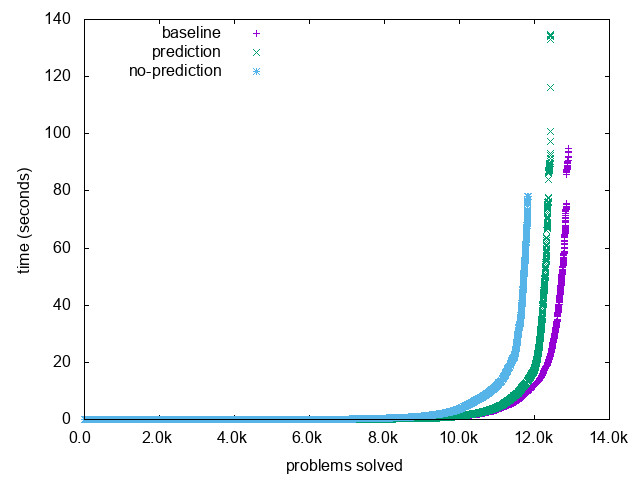
\includegraphics[width=0.6\textwidth]{results.jpeg}
\caption{Plot of problems solved against time for the three variations.\label{fig:results}}
\end{figure}



\begin{table}[t]
\caption{Amount of speedup or slowdown compared to the baseline solver.\label{tab:speedup}}
\centering
\begin{tabular}{l|cc|cc}
		& \multicolumn{2}{c|}{no-prediction} & \multicolumn{2}{c}{prediction} \\ \cline{2-5}
		& wall & cpu & wall & cpu \\ \hline
Average Speedup &1.54 & 6.90 & 1.94 & 6.24 \\ \hline
Number of times better & 451 & 788 & 650 & 1,297 \\
Number of times worse & 1,895 & 2,518 & 642 & 940\\ \hline
Average Speedup (when better) & 7.02 & 28.19 &  3.47& 10.46 \\
Average Slowdown (when worse) & 29.02 & 78.82 & 18.83 & 44.52\\
\end{tabular}
\end{table}

\paragraph{Discussion} An immediate observation is that the overall number of problems solved is slightly worse for the variations performing scheduling. An immediate explanation for this could be that the strategies in the portfolio mode might still be quite fragile i.e. their performance might be degrading with the small overhead of context-switching and additional memory contention. Further experiments could explore this by using more generic strategies with longer individual time limits (many strategies in CASC mode run for less than 1 second). However, the overall number of problems solved is still high enough to make the result useful. The new problems solved by the scheduling variations could also be attributed to this non-determinism, suggesting again that more effort should be spent to provide a broader set of complementary strategies to choose from. We note that one explanation for this second effect could have been if the strategy schedule was longer than the time given and prediction moved a strategy into the allowed time. This is a behaviour we might expect for short time limits but for this experiment all strategies were run.

The average solution times are improved with the two variations and the variation using prediction achieves the best solution time on average. When looking at the more detailed results of Table~\ref{tab:speedup} we see that in the majority of cases the prediction variant was faster than the baseline, which was not the case when no prediction was applied. Furthermore, the impact of getting it wrong was larger without prediction (i.e. the slowdown is bigger).


%%%%%%%%%%%%%%%%%%%%%%%%%%%%%%%%%%%%%%%%%%%%%%%%%%%%%%%
\section{Conclusions and future work} \label{sec:conclusion}
%
The aim of these experiments was to improve Vampire's overall performance, if not in the number of total theorems proved, but in the average time taken to prove problems.
This approach has been shown to produce a significant increase in speed without an excessive penalty in the number of problems solved.

There are several routes that could be explored in order to further improve performance.
As well as improving predictor performance by use of more sophisticated data curation, processing, and machine-learning techniques, it may also be possible to improve the na\"ive scheduling algorithm.
Further research might include designing scheduling algorithms which keep predictions as up-to-date as possible, maximise processor utilisation, minimise memory usage/swapping, reduce context-switching overhead, or even minimise the number of required calls to the prediction algorithm.

This form of optimisation for Vampire is relatively novel: historically the aim of the team has been to prove as many theorems as possible, rather than to improve the speed of moderately-hard problem solving.
As immediate impact, these developments may be useful in improving Vampire's performance in the new SLH division in the CASC competition, as well as improving the overall usability of ITP via quicker ``hammer'' results, such as those reported via Sledgehammer~\cite{sledgehammer}.

\bibliographystyle{plain}
\bibliography{references}
\end{document}
